\documentclass{Group_Templ}

\setlength{\parindent}{0pt}
\begin{document}

\section*{Exercise 7.3}
\begin{enumerate}
	\item 
	\textbf{False.}
	
	Having the same optimal objective value does not imply
	that every optimal LP solution is also feasible for the IP.
	
	Consider the following integer program:
	\begin{align*}
		\max \quad &2x_1+x_2\\
		\text{s.t.}\quad
		2x_1+x_2 &\leq 6,\\
		\frac{1}{2}x_1+x_2 &\leq 3,\\
		x_1,x_2 &\in \mathbb{Z}_{\geq 0}.
	\end{align*}
	
	The optimal integer solution $(3,0)$ achieves
	the objective value
	\[
	z_{\mathrm{IP}}^*=2\cdot3+0=6.
	\]
	
	However, the LP relaxation also has the optimal
	solution $(2.5,1)$, which achieves
	\[
	z_{\mathrm{LP}}^*=2\cdot2.5+1=6.
	\]
	
	Although both programs have the same optimal
	objective value, $(2.5,1)$ is not feasible for
	the IP because $2.5\notin\mathbb{Z}$.
	
	Therefore, the statement is false.

	\item
	\textbf{False.}
	
	An optimal integer solution that is also a vertex of
	the feasible region of the LP relaxation is not
	necessarily optimal for the LP.
	
	Consider the following integer program:
	\begin{align*}
		\max \quad &2x_1+x_2\\
		\text{s.t.}\quad
		2x_1+x_2 &\leq 6.5,\\
		x_1 &\leq 3,\\
		x_1,x_2 &\in \mathbb{Z}_{\geq 0}.
	\end{align*}
	
	The optimal integer solution $(3,0)$ achieves
	the objective value
	\[
	z_{\mathrm{IP}}^*=2\cdot3+0=6.
	\]
	
	Furthermore, $(3,0)$ is a vertex of the feasible
	region of the LP relaxation, since the constraints
	$x_1=3$ and $x_2=0$ intersect at this point.
	
	However, the LP relaxation has the optimal
	solution $(3,0.5)$, which achieves
	\[
	z_{\mathrm{LP}}^*=2\cdot3+0.5=6.5.
	\]
	
	Since
	\[
	z_{\mathrm{LP}}^*>z_{\mathrm{IP}}^*,
	\]
	the optimal integer solution $(3,0)$ is not
	optimal for the LP relaxation.
	
	Therefore, the statement is false.

\end{enumerate}
\section*{Exercise 7.4}

Let $x_{ij}$ indicate whether an edge $(A_i,B_j)$ is selected:
\[
x_{ij}=
\begin{cases}
	1 & \text{if edge }(A_i,B_j)\text{ is selected},\\
	0 & \text{otherwise}.
\end{cases}
\]

\begin{enumerate}
	\item
	The objective is to minimize the total weight of the
	selected edges:
	\[
	\min \sum_{(A_i,B_j)\in E} w_{ij}x_{ij}
	\]
	
	The corresponding primal LP $(P)$ is:
	\begin{align*}
		\min\quad
		&2x_{11}+x_{12}+2x_{21}+x_{22}+3x_{23}\\
		&+2x_{33}+2x_{34}+x_{42}+3x_{43}+3x_{44}\\
		\text{s.t.}\quad
		x_{11}+x_{12}&=1 &&(A_1)\\
		x_{21}+x_{22}+x_{23}&=1 &&(A_2)\\
		x_{33}+x_{34}&=1 &&(A_3)\\
		x_{42}+x_{43}+x_{44}&=1 &&(A_4)\\
		x_{11}+x_{21}&=1 &&(B_1)\\
		x_{12}+x_{22}+x_{42}&=1 &&(B_2)\\
		x_{23}+x_{33}+x_{43}&=1 &&(B_3)\\
		x_{34}+x_{44}&=1 &&(B_4)\\
		x_{ij}&\geq0
		&&\forall(A_i,B_j)\in E.
	\end{align*}
	
	\item
	The corresponding dual LP $(D)$ is:
	\begin{align*}
		\max\quad
		&u_1+u_2+u_3+u_4+v_1+v_2+v_3+v_4\\
		\text{s.t.}\quad
		u_1+v_1&\leq2\\
		u_1+v_2&\leq1\\
		u_2+v_1&\leq2\\
		u_2+v_2&\leq1\\
		u_2+v_3&\leq3\\
		u_3+v_3&\leq2\\
		u_3+v_4&\leq2\\
		u_4+v_2&\leq1\\
		u_4+v_3&\leq3\\
		u_4+v_4&\leq3\\
		u_i,v_j&\in\mathbb{R}
		&&\forall i,j\in\{1,2,3,4\}.
	\end{align*}
	
	\item
	\textbf{Step 1: Initialize the dual variables}
	
	For all A-vertices, set:
	\[
	u_1=u_2=u_3=u_4=0.
	\]
	
	For each B-vertex, choose:
	\[
	v_j=\min_{\substack{i\\(A_i,B_j)\in E}}c_{ij}.
	\]
	
	Therefore:
	\[
	u=(0,0,0,0),\qquad v=(2,1,2,2).
	\]
	
	\textbf{Step 2: Calculate the reduced edge weights}
	
	\[
	w_{ij}=c_{ij}-u_i-v_j
	\]
	
	\begin{align*}
		w_{11}&=2-0-2=0\\
		w_{12}&=1-0-1=0\\
		w_{21}&=2-0-2=0\\
		w_{22}&=1-0-1=0\\
		w_{23}&=3-0-2=1\\
		w_{33}&=2-0-2=0\\
		w_{34}&=2-0-2=0\\
		w_{42}&=1-0-1=0\\
		w_{43}&=3-0-2=1\\
		w_{44}&=3-0-2=1
	\end{align*}
	
	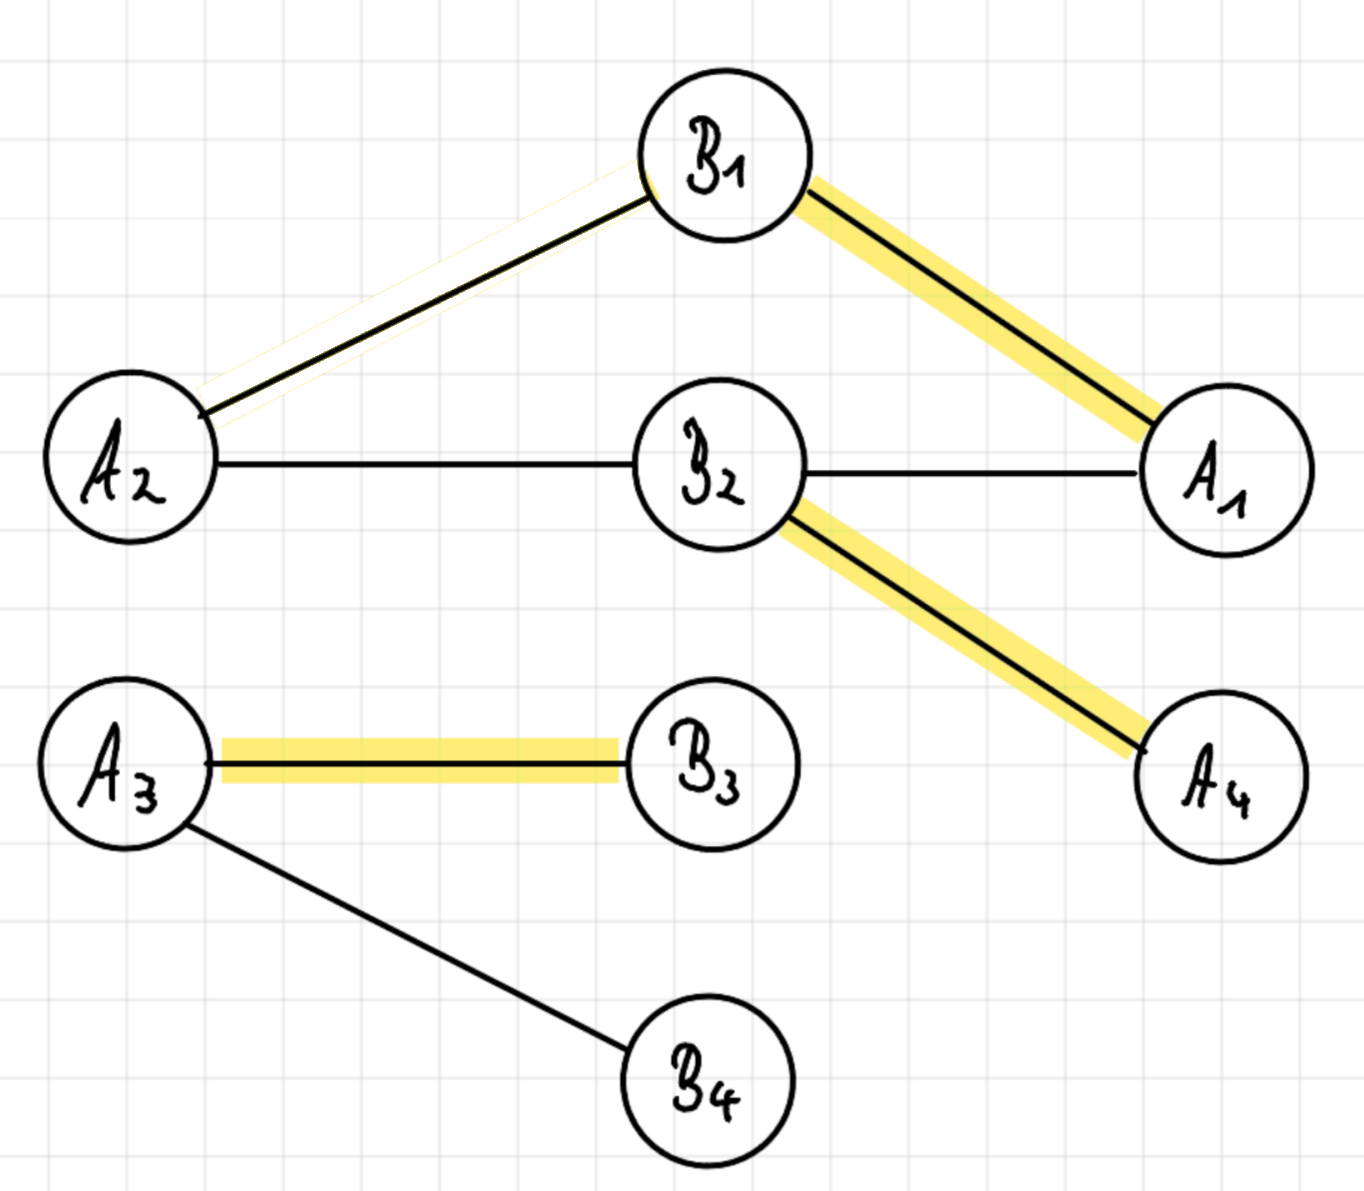
\includegraphics[width=0.7\textwidth]{graph_iteration_1.png}
	\newpage
	\textbf{Step 3: Check for a perfect matching}
	
	The neighbors in the zero-weight graph are:
	\begin{align*}
		A_1&\rightarrow\{B_1,B_2\}\\
		A_2&\rightarrow\{B_1,B_2\}\\
		A_3&\rightarrow\{B_3,B_4\}\\
		A_4&\rightarrow\{B_2\}
	\end{align*}
	
	Consider the subset:
	\[
	X=\{A_1,A_2,A_4\}.
	\]
	
	Its neighborhood is:
	\[
	N(X)=\{B_1,B_2\}.
	\]
	
	Since
	\[
	|X|=3>2=|N(X)|,
	\]
	Hall's condition is violated. Therefore, no perfect
	matching exists in the current zero-weight graph.
	
	A maximum matching is:
	\[
	M=\{(A_1,B_1),(A_4,B_2),(A_3,B_3)\}.
	\]
	
	The vertex $A_2$ remains unmatched.
	
	\textbf{Step 4: Update the dual variables}
	
	Starting from the unmatched vertex $A_2$, the vertices
	reachable by alternating paths are:
	\[
	L=\{A_1,A_2,A_4,B_1,B_2\}.
	\]
	
	Calculate:
	\[
	\delta=
	\min_{\substack{A_i\in A\cap L\\
			B_j\in B\setminus L}}w_{ij}
	\]
	
	\begin{align*}
		\delta
		&=\min\{w_{23},w_{43},w_{44}\}\\
		&=\min\{1,1,1\}\\
		&=1.
	\end{align*}
	
	The dual variables are updated according to:
	\[
	u_i'=
	\begin{cases}
		u_i+\delta & A_i\in L,\\
		u_i & A_i\notin L,
	\end{cases}
	\]
	\[
	v_j'=
	\begin{cases}
		v_j-\delta & B_j\in L,\\
		v_j & B_j\notin L.
	\end{cases}
	\]
	
	The initial values are:
	\[
	u=(0,0,0,0),\qquad v=(2,1,2,2).
	\]
	
	After updating:
	\[
	\boxed{
		u'=(1,1,0,1),\qquad v'=(1,0,2,2)
	}
	\]
	
	\textbf{Second iteration, Step 2: Recalculate the reduced weights}
	
	\[
	w_{ij}'=c_{ij}-u_i'-v_j'
	\]
	
	\begin{align*}
		w_{11}'&=2-1-1=0\\
		w_{12}'&=1-1-0=0\\
		w_{21}'&=2-1-1=0\\
		w_{22}'&=1-1-0=0\\
		w_{23}'&=3-1-2=0\\
		w_{33}'&=2-0-2=0\\
		w_{34}'&=2-0-2=0\\
		w_{42}'&=1-1-0=0\\
		w_{43}'&=3-1-2=0\\
		w_{44}'&=3-1-2=0
	\end{align*}
	
	All existing edges now have a reduced weight of zero.
	
	The resulting graph from Step 2 of the second
	iteration is shown below. All edges in the resulting graph have a reduced weight of zero.
	
	\begin{center}
   		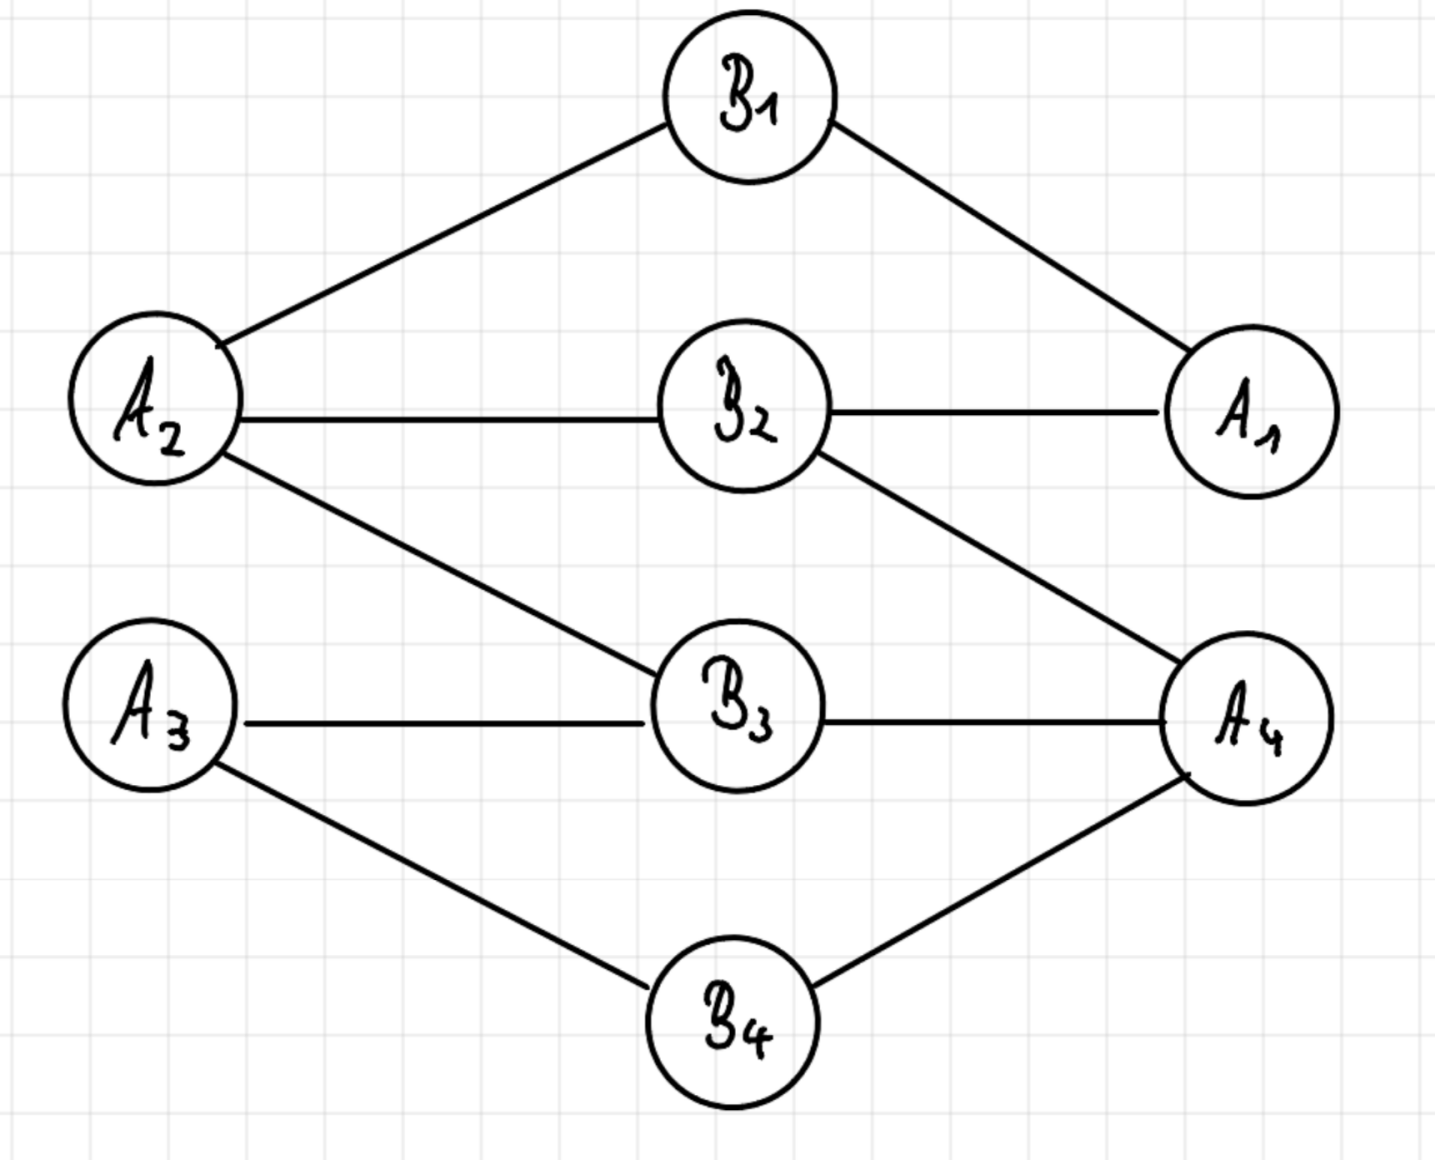
\includegraphics[width=0.75\textwidth]{graph_iteration_2.png}
	\end{center}
	
\end{enumerate}


\end{document}
